\documentclass[a4paper,10pt,fleqn,titlepage,twoside]{article}
\usepackage{amsmath}
\usepackage{graphicx}
\usepackage{epstopdf}
\usepackage[colorlinks,linkcolor=red,urlcolor=red,citecolor=red,plainpages=false,pdfpagelabels,breaklinks]{hyperref}
\pagestyle{plain}
\graphicspath{./img/}

\title{Architecture for a High Speed SAR ADC}
\author{
        Joseph Palackal Mathew \\
	Department of Electrical Engineering\\
        University of California,Los Angeles\\ 
	\href{mailto:jpmathew@ucla.edi}{jpmathew@ucla.edu}
}
\date{\today}
\begin{document}
\maketitle

\section*{Problem Definition}
Derive a topology that will minimize power while achiveing 12 bits of resolution and 200MSPS speed . Make topology amenable for future interleaving 
that can improve speed.

\section*{Problem Analysis}

We are given an input $x\:\epsilon\:[-1,1]$ and converter tries to find K such that $$-1+K\Delta \leq x \leq -1+(K+1)\Delta.$$ If input
is uniformly distributed then the problem will require a minimum $N=log_2(2/\Delta)$ ``Yes or No'' questions with precise answers. From a circuit
perspective ``Yes or No' is that of a comparator comparing input with a threshold with infinite precision. If the
comparison has finite precision i.e it is unreliable for $|inp| < \epsilon $ then at the end of $N$ questions input can be as far as
$\epsilon$ away from the said range.

A typical SAR ADC conversion proceeds as follows . We compare the input with a threshold $V_{th}(k) = r(k)*(x_{max}(k)+x_{min}(k)) + \epsilon(k) $ where it's
guranteed by previous knowledge that $x\:\epsilon\:[x_{max}(k),x_{min}(k)]$.At the end of comparison the input is guaranteed to be in
$[x_{max}(k),V_{th}(k)]$ or $[x_{min}(k),V_{th}(k)]$ so by setting $x_{max}(k+1)$ and $x_{min}(k+1)$ accordingly we can gurantee that range in which 
input can lie $S(k+1)=x_{max}(k+1)-x_{min}(k+1) < S(k)$ provided that we put the thresholds  $V_{th}(k)\:\epsilon[x_{max}(k),x_{min}(k)]$ . This by iteration 
can guarantee that we can locate input to a finite precision in required number of steps.
\newpage
\subsection*{Sampling Circuit}
Noise power due to Differential sampling referred to input
$$P_{noise} = 2*\frac{KT}{Cs}*\frac{Cs+Cp}{Cs}$$
where $Cs$ = sampling cap and $Cp$ = parasitic cap on top-plate , assuming top plate switch is limiting bandwidth and contributing most of noise compared to bottom plate switch . This is a reasonable 
assumption as every attempt will be made to minimize the top plate switch to reduce charge injection offset.
Input referred SNR assuming differential swing of $\pm V_{REF}$
$$SNR = {V_{REF}}^{2}/2*P_{noise}$$
Assuming a shrink of .8 and $V_{REF} = 0.9$,for a noise performance equaling 12 bit quantization noise $$P_{noise}=\Delta^2/12$$$$Cs=600fF$$
\newpage
\subsection*{Clocked Comparator}
\paragraph{}
	In a latched comparator $V_{in}*e^{t/\tau}=VDD$ . For a minimum resolution input $V_{\delta}$ it will need a time $T_{\delta}  = \tau*ln(VDD/V_{\delta})
$.Input greater than $V_{\delta}$ needs time less time to resolve than $T_{\delta}$.An asynchronous ADC uses this fact for optimization by making every comparison time just enough to make
accurate decision by checking output differential level against VDD or timing out after $T_{max}$. Hence $$T_{cmp}=\tau*ln(VDD/V_{in}).$$ This makes the conversion time input dependant and the worst case
comparison time =~ $N^2/2*\tau*ln(2)$ is a two fold improvement in comparison time. But power saving may be significantly higher if actives are powered down after conversion and negligible if all power is dynamic.
For a latch $\tau = Gm/C = \beta*\sqrt(w)/C_{oxl}*W +C_{load}$ . if offset is non critical (SAR) or calibrated (multibit) no optimization is possible in this
end. At higher precision ($V_\delta~=10mV~=8bit$) noise (thermal/capacitive coupling noise $\propto \frac{1}{C}$) from this may become critical and a switch from a noisy to low noise
latch may be required.This will increase W and hence $\tau$.
\paragraph{}
	A Way to improve the comparison time from $O(N^2)$ to $O(N)$ will be to add gain stages in front of the Clocked comparator to the tune of $2^k$ for $k^{th}$ comparison . This will make compartison time 
constant for all clocks making comparison time $N*\tau*ln(2)$ . But this will add to settling portion of converision time and will be a trade off . 
This will automatically improve noise performance w.r.t clocked comparator . 
\paragraph{}
Another option is to add a pipelined clocked comparator to the first one but not wait for it . So output of second latch will be 
$V_{in}*e^{(t1+t2)/\tau}$ making its resolution better . If decision of first and second latch are different it means previous decision was wrong and has to be corrected . It also means that next bit is immaterial and has tobe opposite to
correct decision  . For example if input is 33 current dac level is 32 since input is very small coarse latch gave default value of 0 instead of correct value of 1 and fine latch gave 1 the crrect value . since conversion is allowed to proceed
next threshold used will be 16 and output will be definitely 1 but instead of applying it we applying fine comparator output and its complement 3rd dac theshold 40 instead of 24 which is more precise and in correct range .
\begin{figure}[hp]
\centering
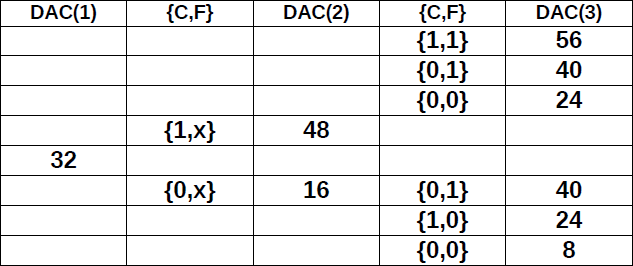
\includegraphics[width=0.95\textwidth]{./img/code.png}
\caption{Code convergance}
\label{fig:pipeCmpCodeConveragnce}
\end{figure}
\begin{figure}[hp]
\centering
\setlength\fboxsep{5.0pt}
\setlength\fboxrule{0.5pt}
\fbox{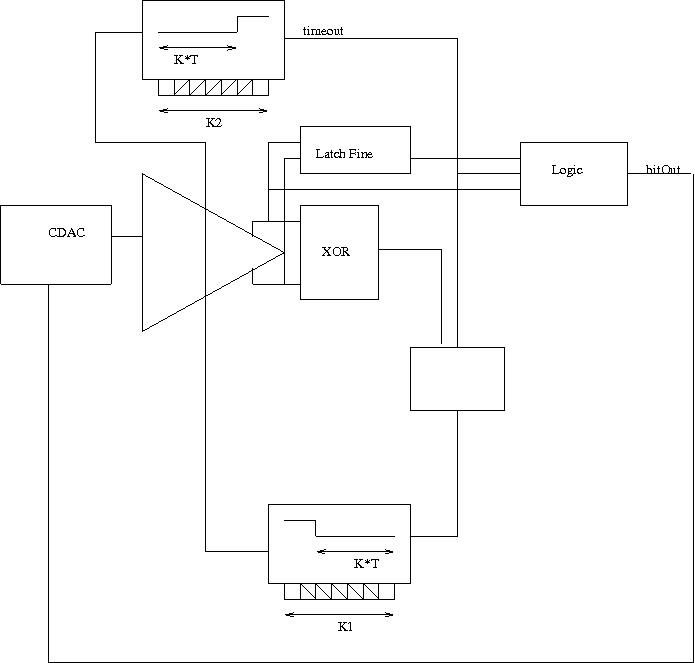
\includegraphics[width=0.95\textwidth]{./img/cmpArch.pdf}}
\caption{scheme}
\label{fig:archReinforce}
\end{figure}
This doesnt improve the performance in terms of O(.) . However since comparator need be only as precise as the next step we will need comparison time of N(N+1)/2 instead of (N+K)*(N+K+1)/2 allowed by redundancy .
In the absense of redundancy this is very significant.The following comparator topology is proposed for implementing either of these schemes
\newpage
\subsection*{Non binary SAR}
\paragraph{}
	In a SAR ADC without any redundancy $k_{th}$ DAC step S(k) needs to settle to $1LSB = VREF/2^{N}$ for ADC to 
to converge correctly . In a constant clock environment this requires a time $T_{dac}=\tau*N*ln(2)$ corresponding to worst case first step and hence a total
DAC time of $\tau*N^{2}*ln(2)$. If each DAC step gets a settling time just enough to meet the settling requirement then $T_{dac}(k)=\tau*(N-k)*ln(2)$ and total dac
time will be $\tau*N(N-1)/2*ln(2)$. To make $T_{DAC}$ a constant we need redundancy propotional to current step so that an error $S(k)*e^{-T_{dac}/\tau}$ can be tolerated
.For this 
\begin{align*}
\sum_{(k+1)}^N{S(i)} &= (1+m)*S(k)\\
\sum_{(k+2)}^N{S(i)} &= (1+m)*S(k+1)\\
S(k+1) &= (1+m)*(S(k)-S(k+1))\\
S(k+1) &= (1+m)/(2+m)*S(k)\\
\end{align*}
This Points to a non binary radix $r=(1+m)/(2+m)$ . since redundancy greater than a step is not required $m<1$ and $r<2/3$. Total conversion clock = $\tau*ln(1/m)*ln(2)*ln(m+1)/ln(2+m)$.
Though this points to a near zero conversion time with m=1 its a mathematical anomally because of approximating error as $S(k)*e^{-T_{dac}/\tau}$ . More correct Derivation
is as follows (assumes non binary sar)
\begin{align*}
settling error &= \sum_1^k{S(i)*e^{(-(k-i)*T_{clk}+T_{dac})/\tau}}\\
S(k)&=1/2*r^{(k-1)}\\
settling error &= 1/2*r^{(k-1)}*e^{-T_{dac})/\tau}*\sum_0^{k-1}{r^{-i}*e^{-iT_{clk}/\tau}}\\
settling error &= 1/2*r^{(k-1)}*e^{-T_{dac})/\tau}*(1-r^{-k}*e^{-k*T_{clk}/\tau})/(1-r^{-1}*e^{-T_{clk}/\tau})\\
e^{-T_{clk}/\tau} &< r for\:Conevergance\\
settling error &~= 1/2*r^{(k-1)}*e^{(-T_{dac}/\tau)}/(1-r^{-1}*e^{-T_{clk}/\tau})\\
settlingerror\:allowed\:by\:redundancy &= m*1/2*r^{(k-1)}\\
T_{clk}&=T_{dac}\Leftarrow\:a\:pessimistic\:approximation\:\\
e^{-T_{dac}/\tau} &= mr/(r+m)\\
r&~=1/2\\
T_{dac} &~= 2*ln(2)*\tau;
\end{align*}
\newpage
\subsection*{Topology}
From analysis of CDAC settling nature and from behavior of comparators if we use non binary SAR we get that 
\begin{align*}
VDD*e^{-T_{cmp}/\tau_1}&+S(k)*e^{-T_{dac}/\tau_2} = S(k)*m\\
\Rightarrow &\;T_{decision}(k) = k*T1+T2\\
\Rightarrow &\;T_{conversion} = N^2*T1+T2*N.
\end{align*}
The $O(N^{2})$ Term in this is what is Causing inefficiency in conversion and cannt be easily avoided without gain . If We add Gain = $2^{k}$ in front
of latch then along with non binary convergance we get latch time to be constant . But the gain component will add a delay which increases linearly 
giving us no merit . This is because this delay element is traversed at each step . Suppose we gain up once and the use it for multiple resolution then
we get a gain . But we still need to settle to required precision if a flash is used . But if a non binary SAR ADC us used and settling is allowed in 
parallel to conversion we can get around this problem . one possible structure for that is as in fig.
\begin{figure}[h]
\centering
\setlength\fboxsep{5.0pt}
\setlength\fboxrule{0.5pt}
\fbox{\includegraphics[width=0.95\textwidth]{./img/ampArch.pdf}}
\caption{topology}
\label{fig:ampArch}
\end{figure}
With finite gain in the amp the voltage at output will be $V_{top}*(1+\Delta))*K$ and hence input referred will be $V_{top}*\Delta$ . Now is P bits are resolved by succeding low precision ADC
$1/(m*r^{k}$  which is quite small and its effect can also be calibrated away and settling should be pretty relaxed as it gets nearly P clocks to reach final value assuming kick back is small . 
Increase in gain is proposed by cascade of stages leading to overall error of the order of $S*\Delta$  for S cascade stages.
\begin{figure}[h]
\centering
\setlength\fboxsep{5.0pt}
\setlength\fboxrule{0.5pt}
\fbox{\includegraphics[width=0.95\textwidth]{./img/ampMulti.pdf}}
\caption{multi Gain Stage configuration}
\label{fig:ampMulti}
\end{figure}
Final Bits will be resolved by normal SAR operation with bits applied every clock on to main CDAC leading to following top level architecture and possible timing as in fig the grouping of bits and 
gain has to be optimized further
\begin{figure}[htbp]
\centering
\setlength\fboxsep{5.0pt}
\setlength\fboxrule{0.5pt}
\fbox{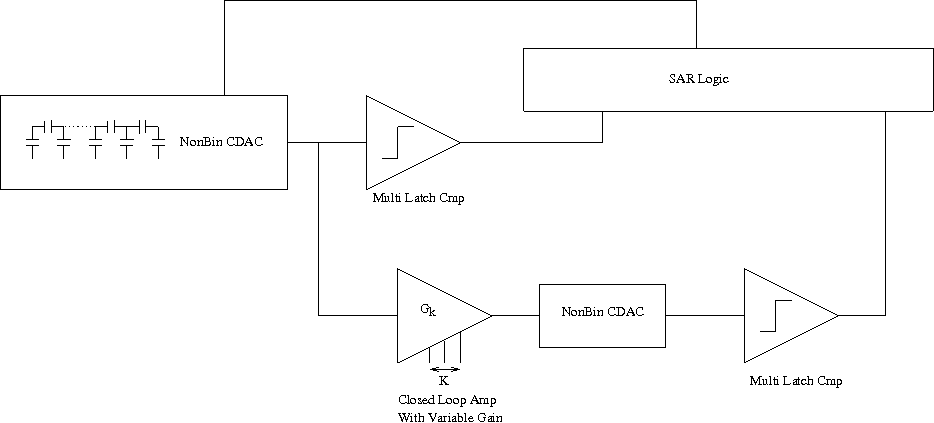
\includegraphics[width=0.95\textwidth]{./img/topArch.pdf}}
\caption{top Level Topology}
\label{fig:topArch}
\end{figure}
\begin{figure}[htbp]
\centering
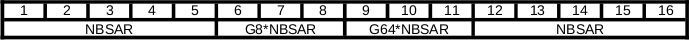
\includegraphics[width=1.0\linewidth]{./img/timing.png}
\caption{One possible conversion pattern}
\label{fig:toptiming}
\end{figure}
\end{document}
